%State Chart Syntax
\section{Syntax of The State Chart Language}

Abstract syntax of our state chart language:

\begin{itemize}
	\item Expression := Expression Op Expression $|$ Op Expression $|$ Variable $|$ Constant
	\item Value := Expression
	\item Type := Char | Int | Long | Bool | Float
	\item Identifier := [a-zA-Z$\_$]+[a-zA-Z0-9$\_$]*  
	
	\item StoreBlock := Type Identifier = Value | Type Identifier = Value; StoreBlock

	\item Condition := Var Eq Var | Var Eq Condition | Condition Eq Condition
	
	\item Eq := $=$ | $\neq$ | $<$ | $\leq$ | $>$ | $\geq$	

	\item StateBlock := StoreBlock	
	
	\item Transition := StateBlock Condition StateBlock
\end{itemize}

\begin{figure}[htp]
    \centering
    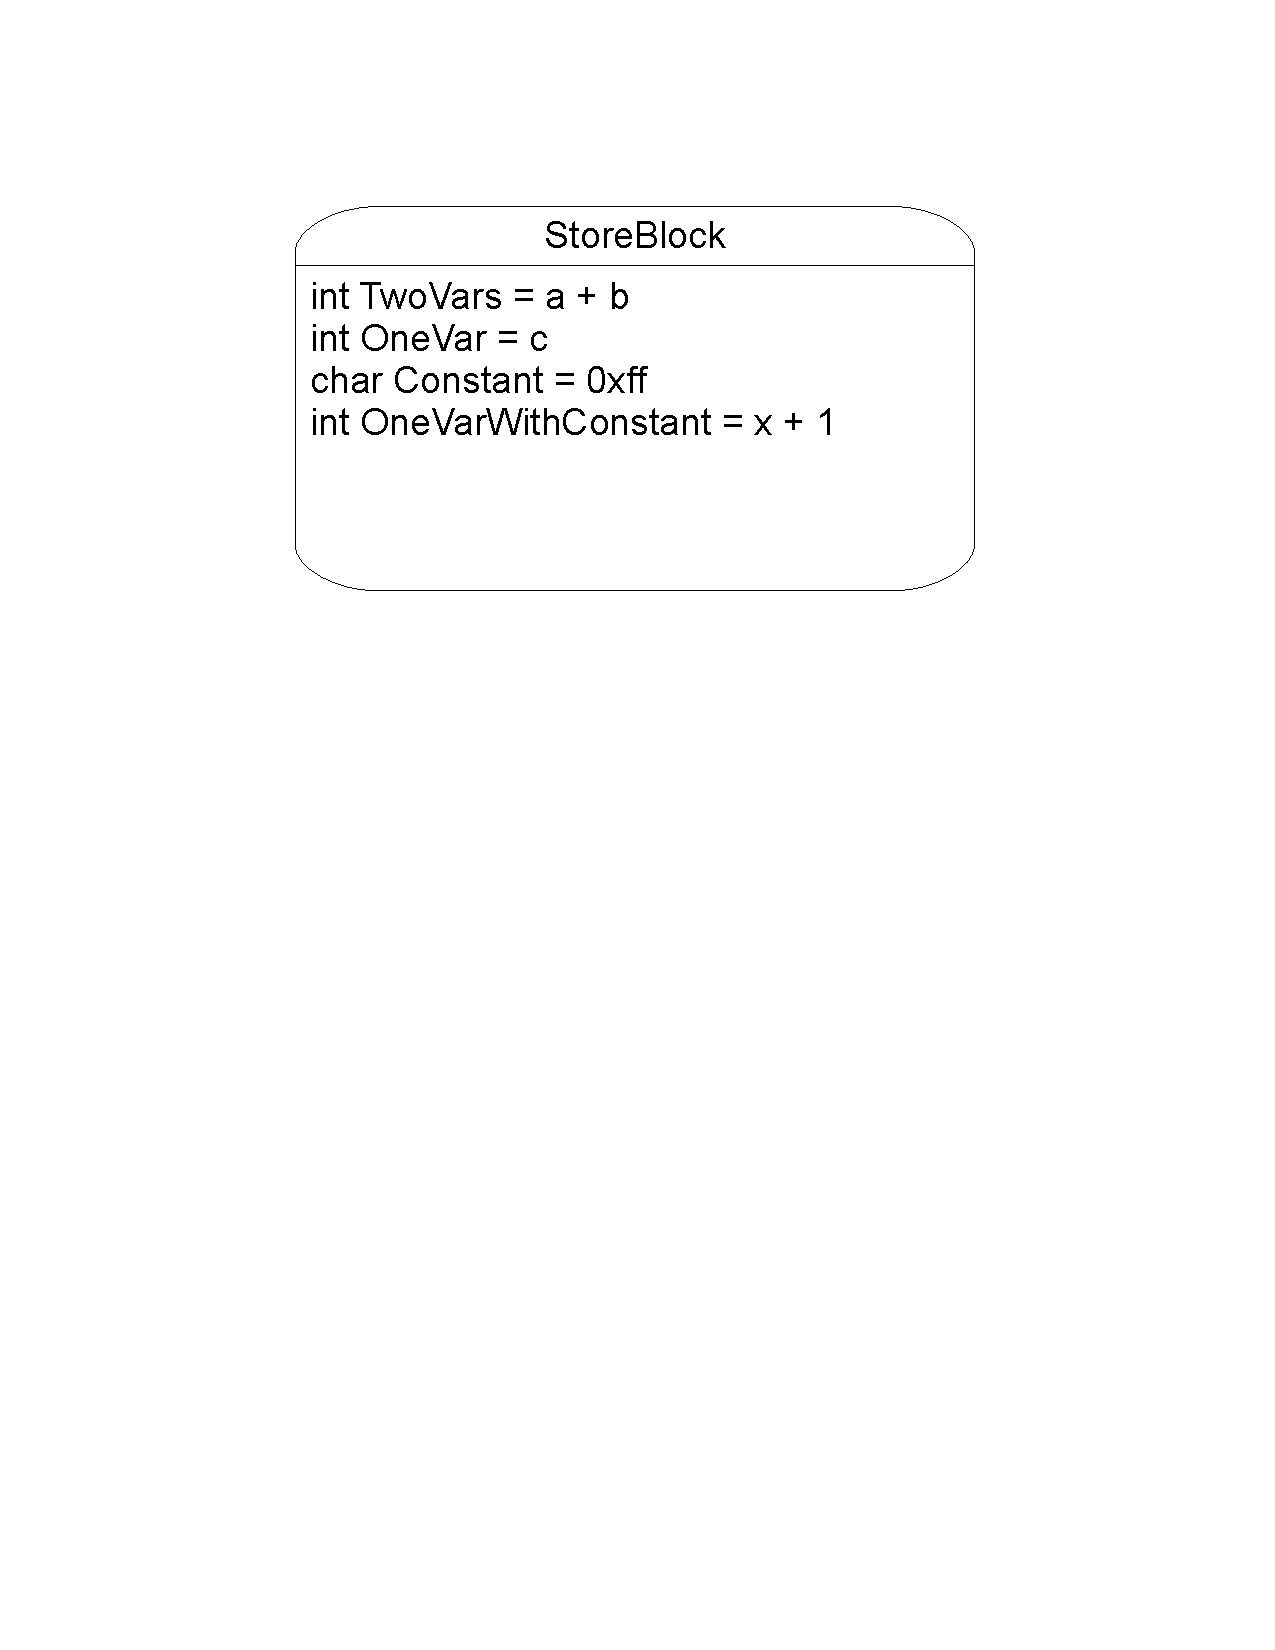
\includegraphics[trim= 20mm 170mm 20mm 10mm, clip, width=\imgmedium]{./images/state_storeblock.pdf}
    \caption{Example Of A Store Block As Implemented In PLCEdit}
    \label{fig:state_storeblock}
\end{figure}

In figure \ref{fig:state_storeblock} we see a store block represented as it would be drawn in the tool. Each line of a store block has the format shown in our abstract syntax. A line consists of a type (which in figure \ref{fig:state_storeblock} we have int, and char) an identifier, the equals symbol, and a value. A value can take the form of several expressions as show in figure \ref{fig:state_storeblock}. Our abstract syntax also allows for many lines to occur in each StoreBlock. This basic design choice allows formulae to be computed much easier in sequence rather than have several blocks to perform one set of operations.

\begin{figure}[htp]
    \centering
    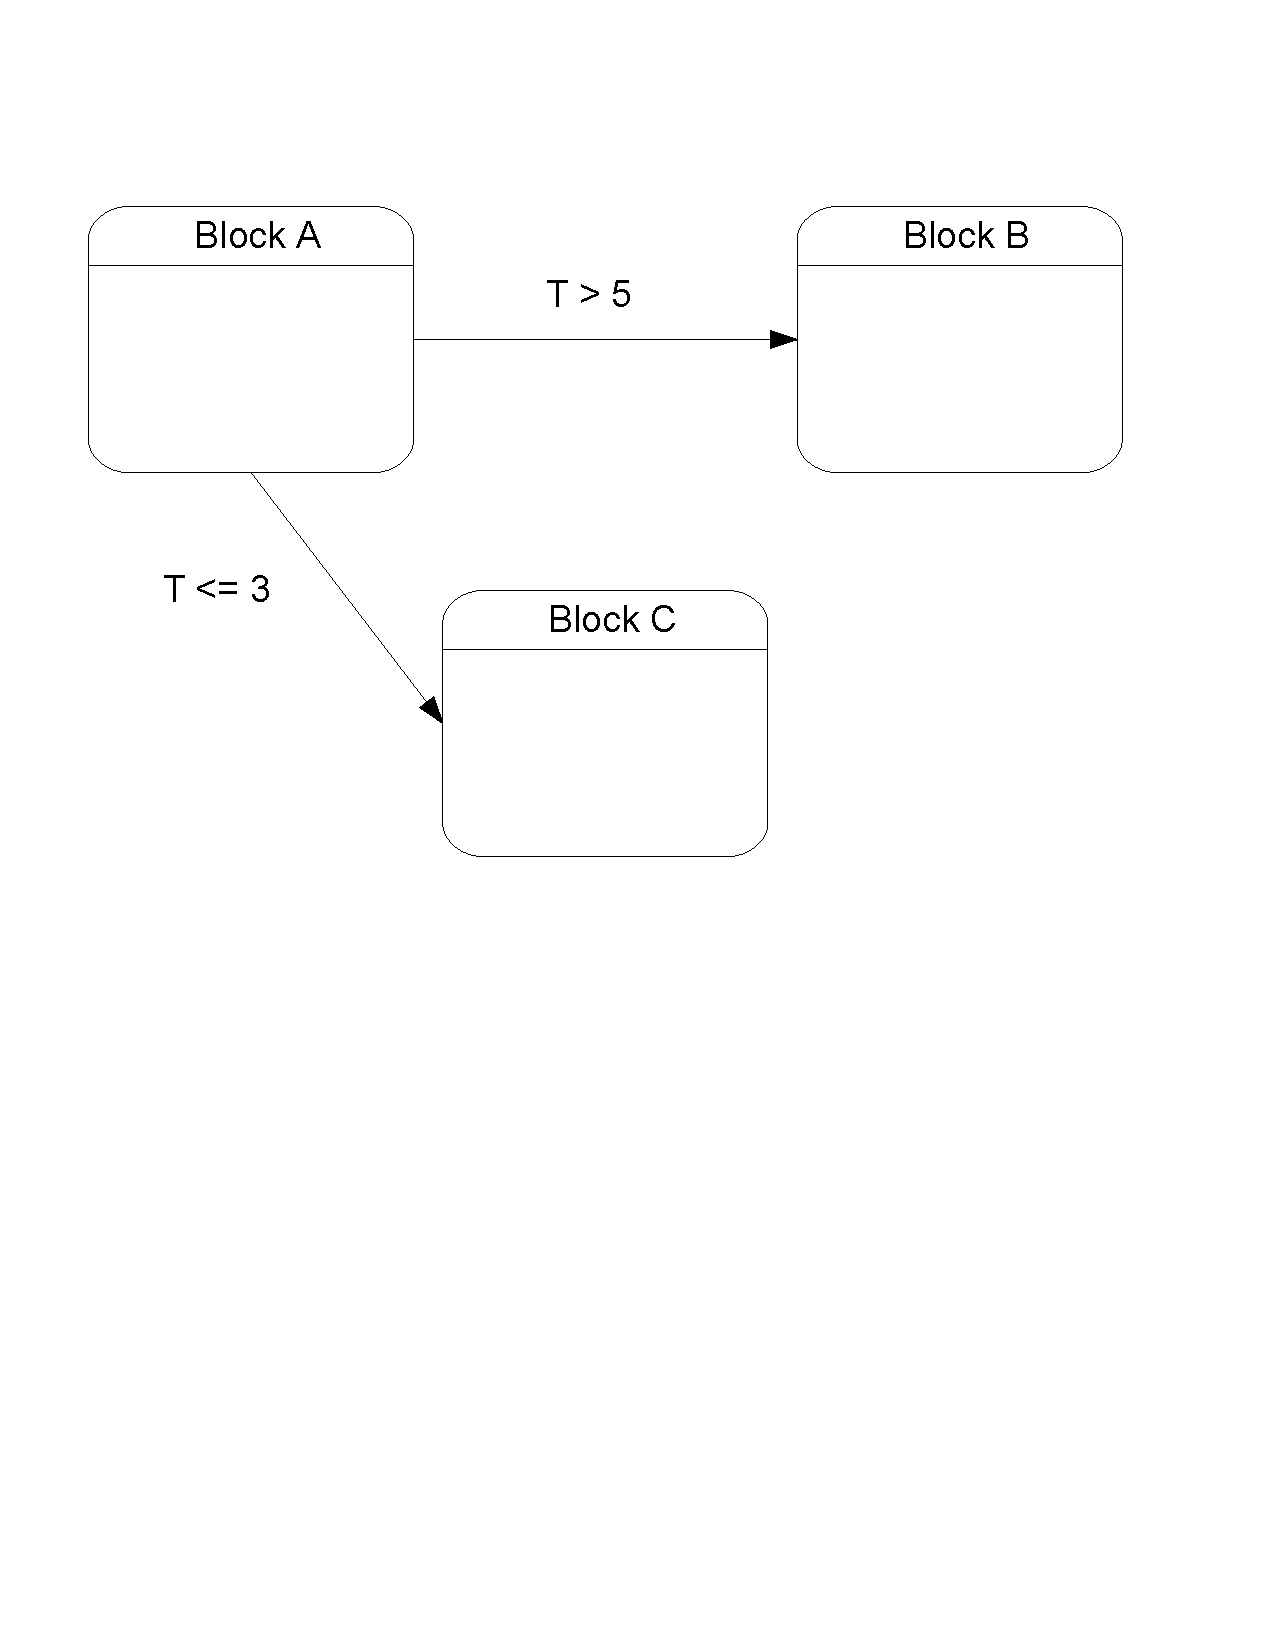
\includegraphics[trim= 10mm 130mm 20mm 10mm, clip, width=\imgmedium]{./images/state_transition.pdf}
    \caption{Example of Basic Transitions}
    \label{fig:state_transition}
\end{figure}

Transitions in our system must start from a  


